\documentclass[a4paper, 12pt]{article}

% Packages
\usepackage[pdftex]{graphicx}
\usepackage{wrapfig}
\usepackage{multicol}
\usepackage[font=small,labelfont=bf,justification=justified,singlelinecheck=false]{caption}
\usepackage{hyperref}
\usepackage{tikz}
\usepackage{listings}
\usepackage{float}

% Fields
\newcommand{\HRule}{\rule{\linewidth}{0.5mm}}
\setlength{\columnsep}{-7.5cm}
\hypersetup{colorlinks, citecolor=black, linkcolor=black, urlcolor=blue}
\tikzstyle{startstop} = [rectangle, rounded corners, text width=3cm, text height=0.3cm, text centered, draw=black, fill=green!20, font=\small]
\tikzstyle{simple} = [rectangle, rounded corners, text width=3cm, text height=0.3cm, text centered, font=\small, draw=black, align=center]
\tikzstyle{option} = [rectangle, rounded corners, dashed, text width=3cm, text height=0.3cm, text centered, font=\small, draw=black, align=center]
\tikzstyle{arrow} = [thick,->,>=stealth]
\tikzstyle{line} = [thick,-,>=stealth]
\lstset{basicstyle=\small\ttfamily, columns=fixed, basewidth=0.48em, fontadjust=true, captionpos=b, numbers=left, frame=single, escapechar=|}

% Document begins
\begin{document}
%---------- title page ----------%
\begin{titlepage}
	\begin{center}
	
\includegraphics[trim = 0mm 0mm 0.2mm 0mm, clip, width=0.6\textwidth]{./uoa-logo}\\[2cm]
	\textsc{\Large Summer Scholarship 2014-2015}\\[0.5cm]
	
	% Title
	\HRule \\[0.4cm]
	{ \LARGE \bfseries Accessible graphics for data on maps \\[0.4cm] }
	\HRule \\[1.5cm]
	
	% Author and supervisor
	\noindent
	\begin{multicols}{2}
		\begin{center}
			\begin{flushleft} \large
		    \emph{Author:} \\
		    \emph{Supervisor:} \\
		    \emph{Degree:} \\
		    \end{flushleft}
		    %
		    \begin{flushleft} \large
		    Eric \textsc{Lim} \\
		    Professor Chris \textsc{Wild} \\
		    \textsc{Honours in Statistics}
		    \end{flushleft}
	  \end{center}
	\end{multicols}
	
	\vfill
	
	% Bottom of the page
	{\large \today}
	
	\end{center}
\end{titlepage}

%---------- experience ----------%
\section*{Summer scholarship experience}
My career objective is to become an independently capable statistician who can design, program and analyse experiments. Personally, I feel that my lack of computer programming skills, along with many others, is an obstacle that must be overcome in order to pursue my lifetime goal. The summer research topic was luckily programming-based to provide me with lots of coding practices and a chance to experience a software development workflow. As I worked my way through I was able to polish up my logical thinking, become a more efficient programmer and learn about the importance of user experience. I am greatly inspired by the summer research to dream of building a statistical software of my own in future.

I would like to thank my supervisor, Professor Chris Wild, for his passionate advices and feedbacks, all of which were invaluable to my career development.

%---------- summary ----------%
\newpage
\section*{Summary}
Statistical analysis is a highly versatile field of study to effectively understand data. It is used in various areas such as finance, ecology, epidemiology and, essentially, any areas that require a set of data to be analysed. In order to perform reasonably satisfying and meaningful analysis, the statistical programming language, \href{http://www.r-project.org/}{R}\footnote{http://www.r-project.org/}, is most preferably and widely used. But is there a way to explore data without having to use lines of computer code?

There are many commercial products to offer statistical features, which may not be ideal for those who only wish to satisfy their statistical curiosity on a smaller scale. Those who are at early stages of learning statistics and only use it on occasions such as for blogging, and even independent statisticians may find these commercial products relatively inaccessible.

For these individuals, the statistical software, \href{https://www.stat.auckland.ac.nz/~wild/iNZight/}{iNZight}\footnote{https://www.stat.auckland.ac.nz/~wild/iNZight/}, may be an option. It is a user-friendly open-source tool to learn statistics and explore various aspects of data. The obstacle of having to learn a programming language is not present in using the software, which means anyone can download it and use it right away. iNZight is constantly updated with new features, one of which is to deal with a particular type of data known as the geographical data.

The geographical data contains positional information, most commonly in the latitude and longitude coordinate system, that provides a way to visualise the geographical information and generate useful insights. In statistics, one of the preferred methods to quickly explore a data set is through visualisation which is exactly what the geographical data most effectively deliver.

To give an example of their usefulness, geographical data can reveal areas of high crime, population, education level and demand for certain products, allowing these \emph{spatial patterns} to be immensely useful in policy making, resource management, marketing, accident monitoring, and emergency planning and routing.

Many of today's technology use location data to provide location-based services such as the GPS tracking that allow us to be more spatially aware of our surroundings and interest us in what may be happening in those areas. I hope that people can use iNZight and its new feature to learn and fulfil their spatial curiosity without a hassle and monetary issue.

The rest of this report includes in-depth discussions of how the new geographical feature is implemented in the software, its limitation and possible future directions.

%---------- abstract ----------%
\newpage
\section*{Abstract}
Geospatial analysis requires our attention as the society is constantly faced with the emergence of various geographical data. It is worthwhile to investigate whether the set of informational techniques used in geospatial analysis can be featured in iNZight. As an initial step, only geographic visualisation has been explored in this project rather than the whole broad field of geospatial analysis. A basic geographic visualisation method is implemented using a recent R package, \textbf{ggmap}. The decision is primarily based on the fact that the package is able to provide visually appealing graphics and offers extensive amount of graphical configuration and flexibility through the philosophy of the grammar of graphics. While achieving the high flexibility, executing a task using this package is quick and fairly light. As a result, the implementation, which we call the \emph{Maps} module, is user-friendly and intuitive to operate, and provides reasonably satisfying graphics as the end product.

%---------- introduction ----------%
\newpage
\section{Introduction}
\label{sec:1}
iNZight is a software which aims to deliver user-friendly and engaging experience in exploring and learning statistics. There are a vast number of future projects for iNZight including multivariate analysis implementation and building a device-independent on-line version. One of the said projects, that this report focuses on, is the implementation of the Geographical Information System (GIS) \cite{tom68}. As a stepping stone, spatial visualisation has been explored because of its effective presentation of geographical data which can quickly reveal geographic patterns and provide intuitive interpretation of those patterns. Under the time constraint and resources available for this project, a basic GIS that presents a set of geographical data on their corresponding locations has been prototyped. The prototype GIS is incorporated in iNZight as a separate module under the \emph{Advanced} tab and is named \emph{Maps} for simplicity. For the rest of the report, the prototype is interchangeably referred to as the Maps module.

%---------- methods ----------%
\section{Methods}
\label{sec:2}
Since this project is essentially about engineering an add-on module to the existing software, the theory of user experience has been highly valued. Mainly the complexity of a workflow and the amount of computational burden, to utilise the new \emph{Maps} module, are aimed to be minimised so that its users can focus on the end product, or the map, itself. This has resulted in a decision to proceed with a raster-based approach rather than a vector-based approach. In-depth reasoning behind the decision is discussed in Section \ref{subsec:2.1}.

There are two main types of basic spatial visualisation; (1) a choropleth and (2) a traditional map. Because of our decision to implement a raster-based visualisation method, only the traditional map implementation could be considered with detailed reasons outlined in Section \ref{subsec:2.2}.

The main algorithm behind the implementation is discussed briefly with a piece of pseudo-code in Section \ref{subsec:2.3}. An intricate discussion is purposely avoided for this section to emphasise the core logic of the implementation method. For the source code of the Maps module, refer to the GitHub repository: \href{https://github.com/iNZightVIT/iNZightMaps}{$\sim$/iNZightVIT/iNZightMaps}.

Lastly, Section \ref{subsec:2.4} includes a concise discussion of the Graphical User Interface of the Maps module.

\subsection{User experience}
\label{subsec:2.1}
An image can exist in two types of graphical formats: (1) the vector graphics, that involves the use of points, lines, curves and polygons based on mathematical expressions, and (2) the raster graphics, that is essentially a rectangular grid of pixels. A vector graphics image is, therefore, scalable as the sizes of the geometrical primitives can be infinitely recalibrated by the mathematical expressions but requires heavier computational processing power and the use of large volumes of data as a result; whereas a raster graphics image is static as each grid of pixels is fixed at the creation of the image resulting in much quicker processing and, therefore, less computational intensity. The main downside of the raster graphics image is that enlarging it above its threshold leads to pixellation that reveals unpleasantly magnified pixels. However, the benefits of using the raster graphics have outweighed those of using the vector graphics in terms of improving the user experience.

The rest of this section discusses the limitations of the vector graphics in regards to improving the quality of the user experience and a set of usable R packages for our chosen visualisation method.

\subsubsection*{Vector-based}
Vector graphics data files encoded with geographical information, such as the popular ESRI Shapefile \cite{esri}, are highly accessible through the web as most of them exist as open-source. However the often large file size, which ranges from tens to hundreds of Megabytes, is problematic for the user experience. Although it seems like a \emph{small} problem in today's standards, the potential waiting period between downloading these files can facilitate inconvenient and frustrating user experience.

In addition, many of iNZight's current users operate it on dated hardware which may not be capable of optimally processing such computationally demanding files.

Another possible obstacle is that many of iNZight's current and future users may be confused with having to import an unfamiliar file format such as the Shapefile, as opposed to the more familiar JPEG or PNG image formats.

Considering all these aspects, the possibility to implement a vector-based visualisation is minimal. Hence a raster-based approach is alternatively examined.

\subsubsection*{Raster-based}
A few packages such as \textbf{maptools} \cite{maptools} and \textbf{rworldmap} \cite{rworldmap} contain geographical boundary data for each country that can be used to produce the world map but can only deliver crude country-specific maps with no display of local boundaries. Hence they were not ideal for visualising geographical data based on a country or a region.

The package, \textbf{dismo} \cite{dismo}, provides wrappers around the \href{http://code.google.com/apis/maps/terms.html}{Google API}\footnote{http://code.google.com/apis/maps/terms.html} for georeferencing and retrieving Google maps. But there were no ways to use the retrieved Google maps as background images on which data points could be plotted. The sole use of \textbf{dismo}'s Google maps was to view them on the R graphics device, which seemed like an unnecessary way to use the Google Maps web-service directly from a browser. The package offered various attractive geospatial modelling methods, all of which were based on the use of vector data files to be unfavourable in this project.

On the contrary, a package called \textbf{ggmap} \cite{ggmap} communicates not only with the Google service but also the \href{http://www.openstreetmap.org/}{OpenStreetMap}\footnote{http://www.openstreetmap.org/}, \href{http://maps.stamen.com/}{Stamen}\footnote{http://maps.stamen.com/} and \href{http://cloudmade.com/}{CloudMade}\footnote{http://cloudmade.com/} services to provide a variety of visually distinctive maps. The philosophy of the grammar of graphics from \textbf{ggplot2} \cite{ggplot2} package is implemented in \textbf{ggmap} to permit manipulation of the grammar of graphics objects and inherit the object-specific options in order to display a highly configurable and visually appealing graphics. Although unnecessary to the Maps module as of yet, \textbf{ggmap} provides other functionalities such as computing distance matrices and time to travel and routes between locations, similar to the GPS tracking service, which may be of potential interest in future. Images retrieved using \textbf{ggmap} are of reasonably high resolution, which means they are less vulnerable to pixellation.

Hence \textbf{ggmap} is the primary resource on which the Maps module is built.

\subsection{Map types}
\label{subsec:2.2}
A choropleth map is a thematic map in which each geographical unit area is shaded or coloured according to the measurement of a representative variable. It provides an intuitive way to visualise how a measurement varies across the area if effective colour progressions are used. However the idea of choropleth map implementation was disregarded because choropleth maps were only available through the use of vector data files in R under the resources and time available for this project.

In addition, choropleth maps can be potentially misused to result in misinterpretation and fabrication of biased information. Firstly, they show a tendency of appealing as if the representative variable is constant across the area, which may present serious issues when (1) the distribution of the variable behaves in an unexpected way and (2) an extreme outlier is associated with the variable. Secondly, the scale of the map limits the depth of inferences that can be made about the variable, i.e., a more detailed inference cannot be made. Thirdly, each area unit does not represent the actual values for the variable but area-weighted values such as percentages and averages that are of no use for forecasting.

Therefore the implementation of choropleth maps has been disregarded.

\subsection{Algorithm}
\label{subsec:2.3}
The Maps module is based on \texttt{draw} function, which is the main method of delivering the raster-based visualisation, with the help of other auxiliary functions. The pseudo-code of the main method is outlined in Listing \ref{lst:1}.

Initially, the geographical bounding box is computed based on the locations in the data set (Line 2) and is, then, used to retrieve the corresponding map from the on-line service of choosing (Line 3). Then, the data set is subsetted according to the range which can be optionally specified on the representative variable (Line 4). Because \textbf{ggmap} has the grammar of graphics implementation, we have decided that it was the most sensible to generate lines of code as text based on the specified graphical settings so that the lines of code can be parsed and evaluated at a later step (Line 6). The retrieved map and the generated lines of code are concatenated together as a \texttt{ggplot} object (Line 7) which is, then, returned to be displayed on the R graphics device (Line 8).

\begin{lstlisting}[caption={\texttt{draw} pseudo-code}, label={lst:1}]
draw = function(data, range, graph_settings, ...) {
	loc = getBB()             # find the bounding box of data
	baseMap = drawMap(loc)    # retrieve a map from online service
	dat = varSubset(range)    # subset data for specified range
	
	l = generateLine(graph_settings)    # generate a line of code
	map = baseMap + l                   # parse the generated line
	return(map)                         # display the map object
}
\end{lstlisting}

\subsection{Graphical User Interface}
\label{subsec:2.4}
The GUI of the Maps module has seen numerous design changes. At the earlier stages of the project, the GUI was designed as a separate window detached from the main iNZight GUI. This was to maximise the usability of the Maps module by providing a diversity of options for more configurable graphics. Towards the end of the project, the Maps GUI is simplified by replacing some of the redundant options with automated processes that choose the options for the users based on the data. For example, a text box that requires user input for the name of the geographical location, which is used to compute the bounding box, is replaced with an automated searching of the location based on the data. Eventually, the Maps GUI is simplified to the extent that it resides as a part of the main iNZight GUI.

%---------- results ----------%
\section{Results}

\begin{figure}[H]
	\centering
	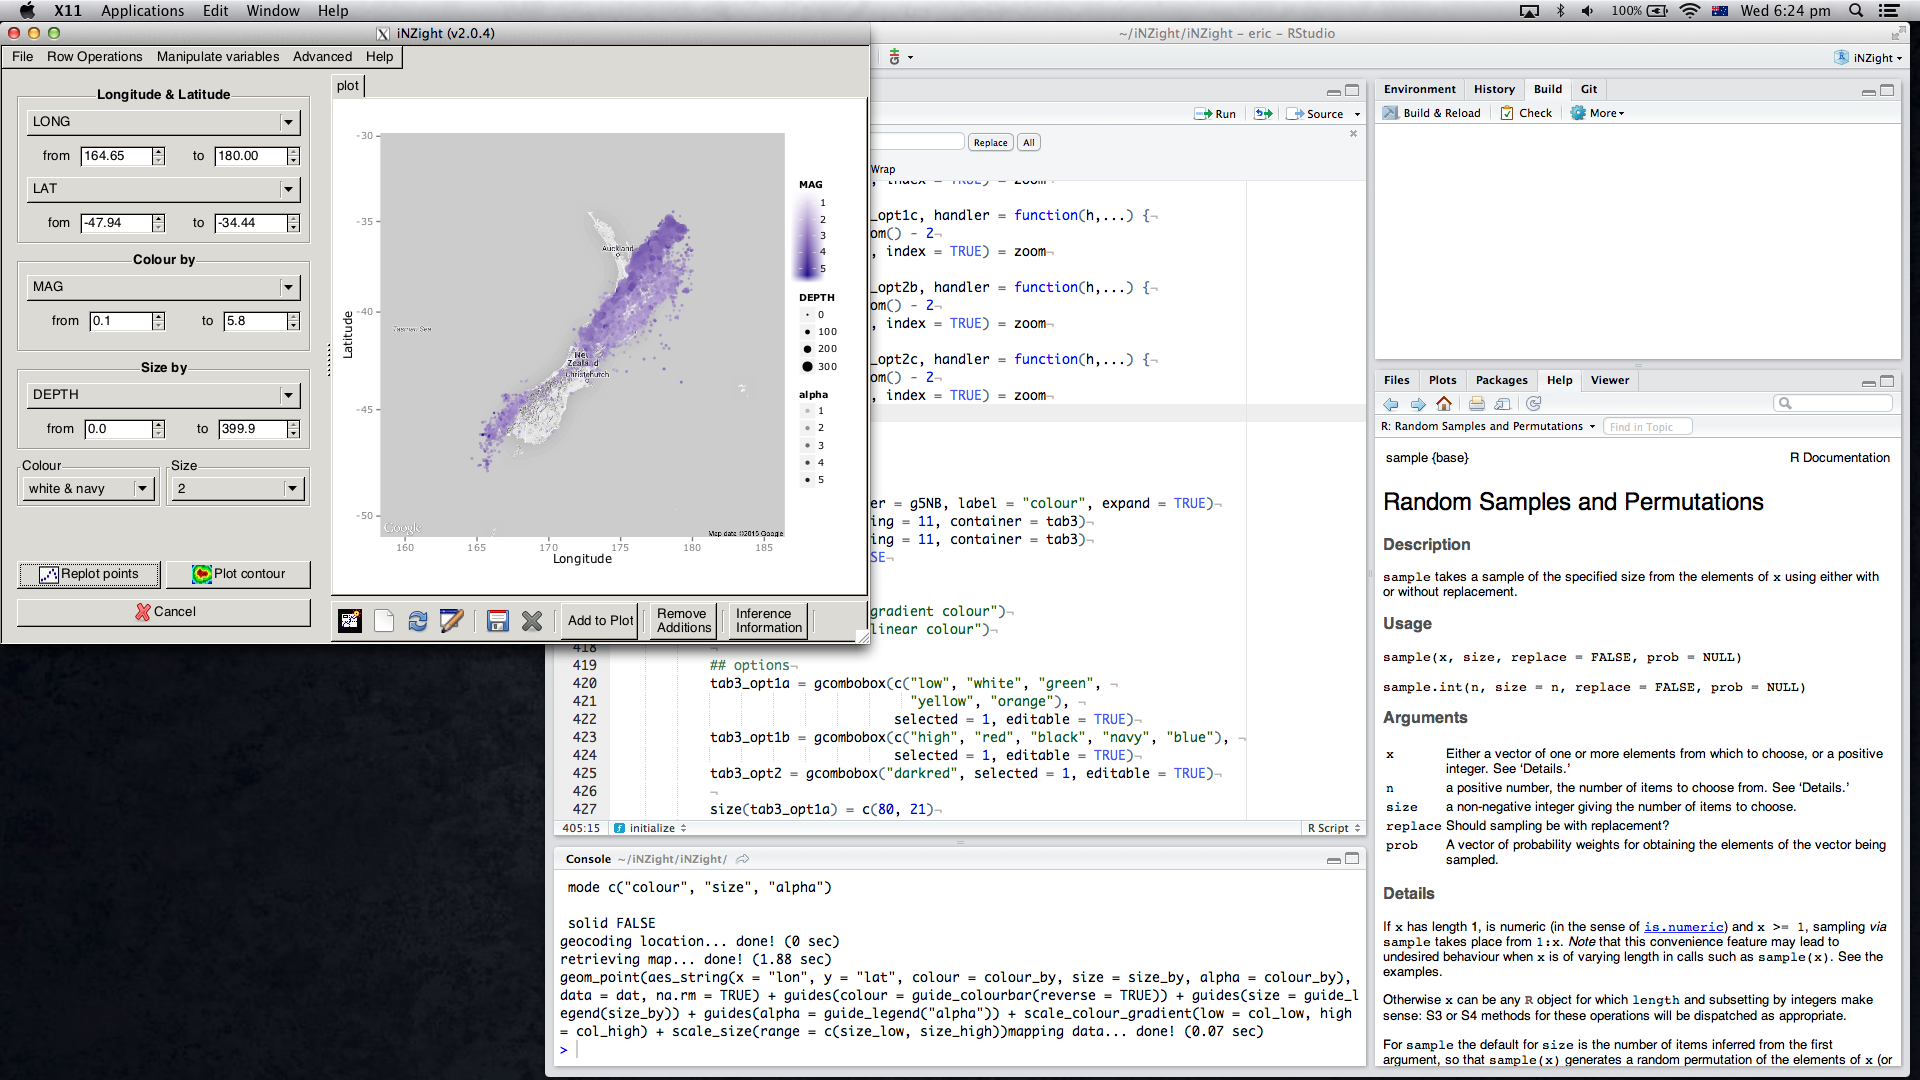
\includegraphics[trim=0cm 15.32cm 37cm 0.72cm, clip, width=1\textwidth]{demo1}
	\caption{2007 New Zealand earthquake data. LONG, LAT, MAG and DEPTH represent the longitude, latitude, magnitude and depth of the earthquakes, respectively.}
	\label{fig:1}
\end{figure}

Figure \ref{fig:1} represents the Maps module along with an output map.

The left side of the GUI is the integrated module which can be closed off to display the default Data View window by clicking the `Cancel' button. For the `\textbf{Longitude and Latitude}' section, each variable in the data set is tested whether the values are in possible longitudinal and latitudinal ranges as well as regular expression-based text matching to computationally select the longitude and latitude variables. The `\textbf{Colour by}' and `\textbf{Size by}' sections are optional for choosing representative variables by which the plotting symbols are scaled.

The right side of the GUI is the R graphics widget to display the graphical output. The plot seen in Figure \ref{fig:1} displays the earthquake data coloured by the order of the magnitude and the size of the plotting symbols are scaled by the order of the depth.

Categorical variables and 2D estimation contours can also be plotted as seen in Figures \ref{fig:2} and \ref{fig:3}, respectively.

\begin{figure}[H]
	\centering
	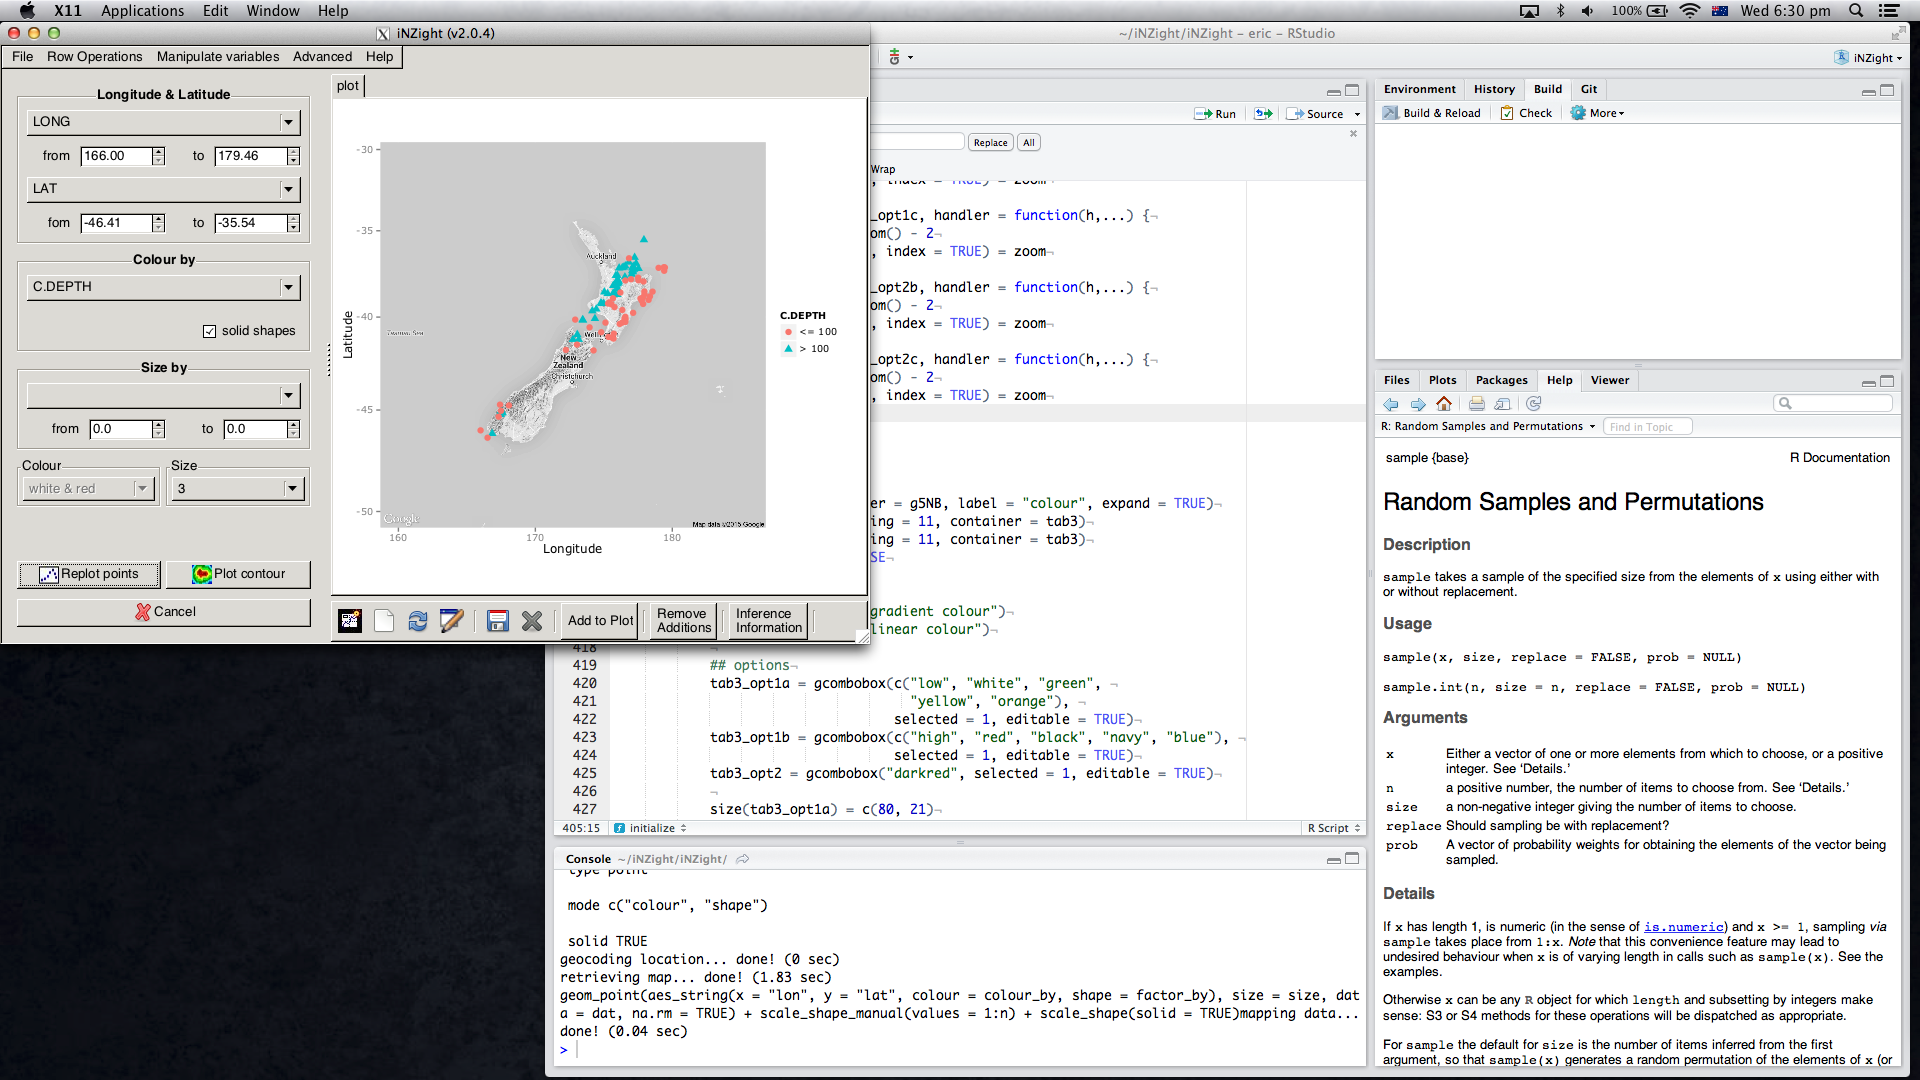
\includegraphics[trim=0cm 15.32cm 37cm 0.72cm, clip, width=0.8\textwidth]{demo3}
	\caption{A random sample of 100 observations is selected from the earthquake data set, where each half of the sample satisfies each condition to avoid overplotting.}
	\label{fig:2}
\end{figure}

\begin{figure}[H]
	\centering
	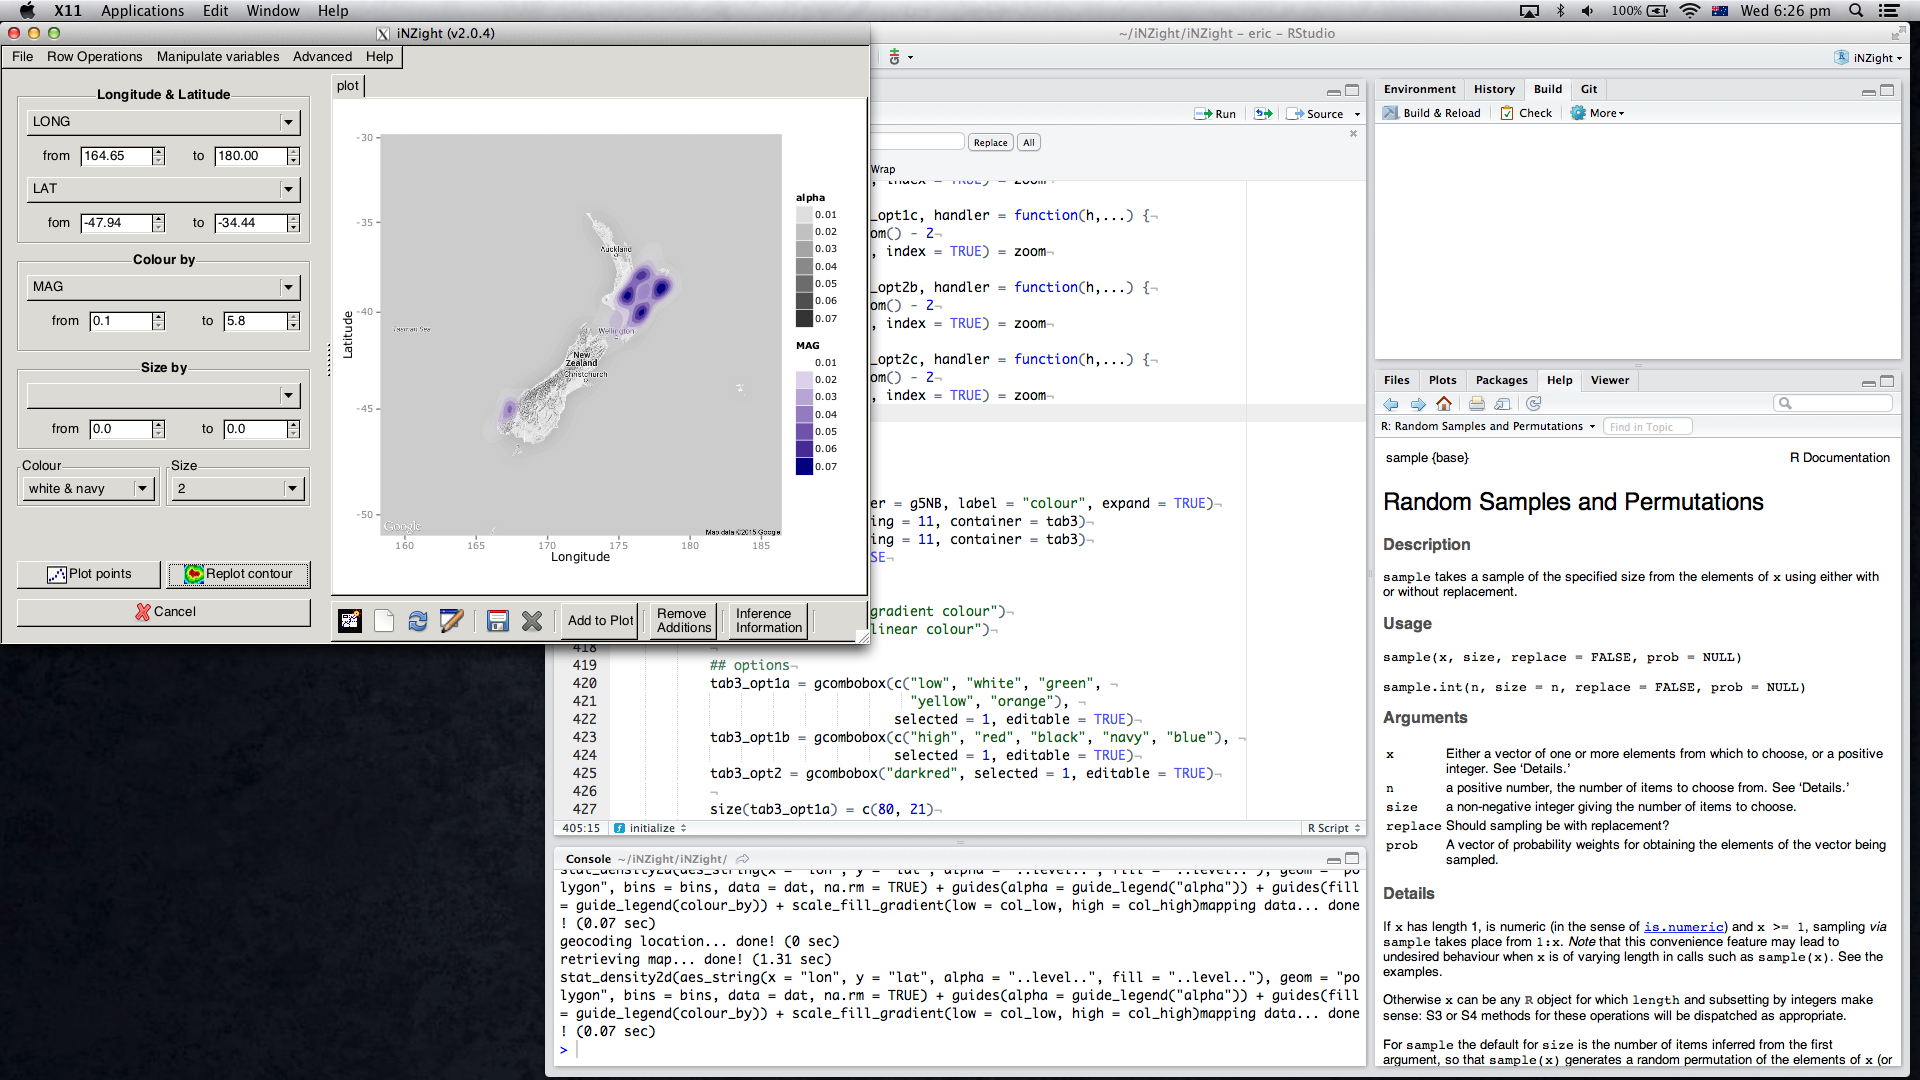
\includegraphics[trim=0cm 15.32cm 37cm 0.72cm, clip, width=0.8\textwidth]{demo2}
	\caption{2D estimation contour of the earthquake data.}
	\label{fig:3}
\end{figure}


%---------- conclusions ----------%
\section{Conclusions}
The Maps module is a basic prototype whose aim is to demonstrate the possibility of implementing spatial visualisation in iNZight. It has demonstrated that the visualisation of geographical data is feasible through the raster-based methodology.

A major limiting factor of the Maps module is the requirement for internet access. Because it communicates with the on-line service, internet access has to be constantly provided throughout the use.

Additionally, the communication process is dependent on the quality of the internet access, such as the speed, as well as the amount of traffic experienced by the on-line service. A note to be considered is that the average time of a complete operation cycle is about 2 seconds which is a much smaller figure compared to the alternative vector data processing time.

User feedbacks have not been available at the completion of this project, which could have been worthwhile to be assessed and discussed.

Possible future directions include: (1) improving the Maps module so that other useful types of plots such as a histogram or a time-series plot could be displayed simultaneously to provide more information rich graphics, (2) exploring raster data formats such as the Esri Grid for better performance and (3) extending the module to be a part of a larger GIS module where other geospatial analysis methods are available.

%---------- references ----------%
\section{References}
\renewcommand{\section}[2]{}%
\bibliographystyle{ieeetr}
\bibliography{ref}

\end{document}